\documentclass[twoside]{book}

% Packages required by doxygen
\usepackage{fixltx2e}
\usepackage{calc}
\usepackage{doxygen}
\usepackage[export]{adjustbox} % also loads graphicx
\usepackage{graphicx}
\usepackage[utf8]{inputenc}
\usepackage{makeidx}
\usepackage{multicol}
\usepackage{multirow}
\PassOptionsToPackage{warn}{textcomp}
\usepackage{textcomp}
\usepackage[nointegrals]{wasysym}
\usepackage[table]{xcolor}

% Font selection
\usepackage[T1]{fontenc}
\usepackage[scaled=.90]{helvet}
\usepackage{courier}
\usepackage{amssymb}
\usepackage{sectsty}
\renewcommand{\familydefault}{\sfdefault}
\allsectionsfont{%
  \fontseries{bc}\selectfont%
  \color{darkgray}%
}
\renewcommand{\DoxyLabelFont}{%
  \fontseries{bc}\selectfont%
  \color{darkgray}%
}
\newcommand{\+}{\discretionary{\mbox{\scriptsize$\hookleftarrow$}}{}{}}

% Page & text layout
\usepackage{geometry}
\geometry{%
  a4paper,%
  top=2.5cm,%
  bottom=2.5cm,%
  left=2.5cm,%
  right=2.5cm%
}
\tolerance=750
\hfuzz=15pt
\hbadness=750
\setlength{\emergencystretch}{15pt}
\setlength{\parindent}{0cm}
\setlength{\parskip}{0.2cm}
\makeatletter
\renewcommand{\paragraph}{%
  \@startsection{paragraph}{4}{0ex}{-1.0ex}{1.0ex}{%
    \normalfont\normalsize\bfseries\SS@parafont%
  }%
}
\renewcommand{\subparagraph}{%
  \@startsection{subparagraph}{5}{0ex}{-1.0ex}{1.0ex}{%
    \normalfont\normalsize\bfseries\SS@subparafont%
  }%
}
\makeatother

% Headers & footers
\usepackage{fancyhdr}
\pagestyle{fancyplain}
\fancyhead[LE]{\fancyplain{}{\bfseries\thepage}}
\fancyhead[CE]{\fancyplain{}{}}
\fancyhead[RE]{\fancyplain{}{\bfseries\leftmark}}
\fancyhead[LO]{\fancyplain{}{\bfseries\rightmark}}
\fancyhead[CO]{\fancyplain{}{}}
\fancyhead[RO]{\fancyplain{}{\bfseries\thepage}}
\fancyfoot[LE]{\fancyplain{}{}}
\fancyfoot[CE]{\fancyplain{}{}}
\fancyfoot[RE]{\fancyplain{}{\bfseries\scriptsize Generated on Wed Dec 16 2015 13\+:44\+:38 for My Project by Doxygen }}
\fancyfoot[LO]{\fancyplain{}{\bfseries\scriptsize Generated on Wed Dec 16 2015 13\+:44\+:38 for My Project by Doxygen }}
\fancyfoot[CO]{\fancyplain{}{}}
\fancyfoot[RO]{\fancyplain{}{}}
\renewcommand{\footrulewidth}{0.4pt}
\renewcommand{\chaptermark}[1]{%
  \markboth{#1}{}%
}
\renewcommand{\sectionmark}[1]{%
  \markright{\thesection\ #1}%
}

% Indices & bibliography
\usepackage{natbib}
\usepackage[titles]{tocloft}
\setcounter{tocdepth}{3}
\setcounter{secnumdepth}{5}
\makeindex

% Hyperlinks (required, but should be loaded last)
\usepackage{ifpdf}
\ifpdf
  \usepackage[pdftex,pagebackref=true]{hyperref}
\else
  \usepackage[ps2pdf,pagebackref=true]{hyperref}
\fi
\hypersetup{%
  colorlinks=true,%
  linkcolor=blue,%
  citecolor=blue,%
  unicode%
}

% Custom commands
\newcommand{\clearemptydoublepage}{%
  \newpage{\pagestyle{empty}\cleardoublepage}%
}


%===== C O N T E N T S =====

\begin{document}

% Titlepage & ToC
\hypersetup{pageanchor=false,
             bookmarks=true,
             bookmarksnumbered=true,
             pdfencoding=unicode
            }
\pagenumbering{roman}
\begin{titlepage}
\vspace*{7cm}
\begin{center}%
{\Large My Project }\\
\vspace*{1cm}
{\large Generated by Doxygen 1.8.10}\\
\vspace*{0.5cm}
{\small Wed Dec 16 2015 13:44:38}\\
\end{center}
\end{titlepage}
\clearemptydoublepage
\tableofcontents
\clearemptydoublepage
\pagenumbering{arabic}
\hypersetup{pageanchor=true}

%--- Begin generated contents ---
\chapter{Hierarchical Index}
\section{Class Hierarchy}
This inheritance list is sorted roughly, but not completely, alphabetically\+:\begin{DoxyCompactList}
\item \contentsline{section}{Avatar}{\pageref{class_avatar}}{}
\item \contentsline{section}{Avatar\+Test}{\pageref{class_avatar_test}}{}
\item \contentsline{section}{Backpack}{\pageref{class_backpack}}{}
\item \contentsline{section}{Backpack\+Test}{\pageref{class_backpack_test}}{}
\item \contentsline{section}{Course}{\pageref{class_course}}{}
\item \contentsline{section}{Creature}{\pageref{class_creature}}{}
\begin{DoxyCompactList}
\item \contentsline{section}{Student}{\pageref{class_student}}{}
\item \contentsline{section}{Teacher}{\pageref{class_teacher}}{}
\end{DoxyCompactList}
\item \contentsline{section}{Creature\+Test}{\pageref{class_creature_test}}{}
\item \contentsline{section}{Gameplay}{\pageref{class_gameplay}}{}
\item \contentsline{section}{Item}{\pageref{class_item}}{}
\begin{DoxyCompactList}
\item \contentsline{section}{Book}{\pageref{class_book}}{}
\item \contentsline{section}{Key}{\pageref{class_key}}{}
\end{DoxyCompactList}
\item \contentsline{section}{Room}{\pageref{class_room}}{}
\item \contentsline{section}{Room\+Test}{\pageref{class_room_test}}{}
\item \contentsline{section}{Sfinxen}{\pageref{class_sfinxen}}{}
\item \contentsline{section}{Sfinxen\+Test}{\pageref{class_sfinxen_test}}{}
\item \contentsline{section}{World}{\pageref{class_world}}{}
\item \contentsline{section}{World\+Test}{\pageref{class_world_test}}{}
\end{DoxyCompactList}

\chapter{Class Index}
\section{Class List}
Here are the classes, structs, unions and interfaces with brief descriptions\+:\begin{DoxyCompactList}
\item\contentsline{section}{\hyperlink{class_customer}{Customer} }{\pageref{class_customer}}{}
\item\contentsline{section}{\hyperlink{class_customer_test}{Customer\+Test} }{\pageref{class_customer_test}}{}
\item\contentsline{section}{\hyperlink{class_queue_1_1_node}{Queue$<$ T $>$.\+Node$<$ E $>$} }{\pageref{class_queue_1_1_node}}{}
\item\contentsline{section}{\hyperlink{class_queue}{Queue$<$ T $>$} }{\pageref{class_queue}}{}
\item\contentsline{section}{\hyperlink{class_queue_test}{Queue\+Test} }{\pageref{class_queue_test}}{}
\item\contentsline{section}{\hyperlink{class_register}{Register} }{\pageref{class_register}}{}
\item\contentsline{section}{\hyperlink{class_simulation}{Simulation} }{\pageref{class_simulation}}{}
\item\contentsline{section}{\hyperlink{class_simulator}{Simulator} }{\pageref{class_simulator}}{}
\item\contentsline{section}{\hyperlink{class_store}{Store} }{\pageref{class_store}}{}
\end{DoxyCompactList}

\chapter{Class Documentation}
\hypertarget{class_avatar}{}\section{Avatar Class Reference}
\label{class_avatar}\index{Avatar@{Avatar}}
\subsection*{Public Member Functions}
\begin{DoxyCompactItemize}
\item 
\hypertarget{class_avatar_a1e169a41bf3a7d8f4bfbff5f141f325a}{}{\bfseries Avatar} (\hyperlink{class_course}{Course}\mbox{[}$\,$\mbox{]} finished, int backpack\+Size, int starting\+H\+P)\label{class_avatar_a1e169a41bf3a7d8f4bfbff5f141f325a}

\item 
\hypertarget{class_avatar_ac874154104cac8c626228fa00324136c}{}boolean {\bfseries add\+New\+Course} (\hyperlink{class_course}{Course} course)\label{class_avatar_ac874154104cac8c626228fa00324136c}

\item 
\hypertarget{class_avatar_a863cde0a614b62439592a4fdeb616456}{}boolean {\bfseries finish\+Course} (\hyperlink{class_course}{Course} course)\label{class_avatar_a863cde0a614b62439592a4fdeb616456}

\item 
\hypertarget{class_avatar_a677b7fba74b8d4092b2255efdb861c9a}{}void {\bfseries print\+Finished\+Courses} ()\label{class_avatar_a677b7fba74b8d4092b2255efdb861c9a}

\item 
\hypertarget{class_avatar_a3a1e90e2daef67f7a5bbdc0faf22639f}{}void {\bfseries print\+Unfinished\+Courses} ()\label{class_avatar_a3a1e90e2daef67f7a5bbdc0faf22639f}

\item 
\hypertarget{class_avatar_a52d8e9edc6db97535eb75ebc753ae418}{}boolean {\bfseries add\+To\+Backpack} (\hyperlink{class_item}{Item} c)\label{class_avatar_a52d8e9edc6db97535eb75ebc753ae418}

\item 
\hypertarget{class_avatar_a2fc1510fbc965e53bfe3e5f43f2ece5b}{}\hyperlink{class_item}{Item} {\bfseries get\+From\+Backpack} (String item\+Name)\label{class_avatar_a2fc1510fbc965e53bfe3e5f43f2ece5b}

\item 
\hypertarget{class_avatar_ae639c0e572b3430f319ef5145a33ec1d}{}int {\bfseries get\+H\+P} ()\label{class_avatar_ae639c0e572b3430f319ef5145a33ec1d}

\end{DoxyCompactItemize}


The documentation for this class was generated from the following file\+:\begin{DoxyCompactItemize}
\item 
Avatar.\+java\end{DoxyCompactItemize}

\hypertarget{class_avatar_test}{}\section{Avatar\+Test Class Reference}
\label{class_avatar_test}\index{Avatar\+Test@{Avatar\+Test}}
\subsection*{Static Public Member Functions}
\begin{DoxyCompactItemize}
\item 
\hypertarget{class_avatar_test_a43a1780e5c1895d7280134919d929372}{}static void {\bfseries main} (String args\mbox{[}$\,$\mbox{]})\label{class_avatar_test_a43a1780e5c1895d7280134919d929372}

\end{DoxyCompactItemize}


The documentation for this class was generated from the following file\+:\begin{DoxyCompactItemize}
\item 
Avatar\+Test.\+java\end{DoxyCompactItemize}

\hypertarget{class_backpack}{}\section{Backpack Class Reference}
\label{class_backpack}\index{Backpack@{Backpack}}
\subsection*{Public Member Functions}
\begin{DoxyCompactItemize}
\item 
\hypertarget{class_backpack_a0133aab8842753b7e15e44ae1405b98e}{}{\bfseries Backpack} (int max\+Size)\label{class_backpack_a0133aab8842753b7e15e44ae1405b98e}

\item 
\hypertarget{class_backpack_ab6659457290a3589e69d50cdd12f0d1b}{}\hyperlink{class_item}{Item} {\bfseries get\+Item} (String name)\label{class_backpack_ab6659457290a3589e69d50cdd12f0d1b}

\item 
\hypertarget{class_backpack_af9628f7226b55d9c97659f230af73d41}{}boolean {\bfseries add\+Item} (\hyperlink{class_item}{Item} item)\label{class_backpack_af9628f7226b55d9c97659f230af73d41}

\item 
\hypertarget{class_backpack_a8860f8d3603fa6cefe41f93fcd23a4f6}{}boolean {\bfseries drop\+Item} (String name)\label{class_backpack_a8860f8d3603fa6cefe41f93fcd23a4f6}

\item 
\hypertarget{class_backpack_a7b9fc10f9aa368b40828d169fc7aaf08}{}void {\bfseries print} ()\label{class_backpack_a7b9fc10f9aa368b40828d169fc7aaf08}

\end{DoxyCompactItemize}


The documentation for this class was generated from the following file\+:\begin{DoxyCompactItemize}
\item 
Backpack.\+java\end{DoxyCompactItemize}

\hypertarget{class_backpack_test}{}\section{Backpack\+Test Class Reference}
\label{class_backpack_test}\index{Backpack\+Test@{Backpack\+Test}}
\subsection*{Static Public Member Functions}
\begin{DoxyCompactItemize}
\item 
\hypertarget{class_backpack_test_aebaf9b3ce7f692226da1a603c4c15379}{}static void {\bfseries main} (String args\mbox{[}$\,$\mbox{]})\label{class_backpack_test_aebaf9b3ce7f692226da1a603c4c15379}

\end{DoxyCompactItemize}


The documentation for this class was generated from the following file\+:\begin{DoxyCompactItemize}
\item 
Backpack\+Test.\+java\end{DoxyCompactItemize}

\hypertarget{class_book}{}\section{Book Class Reference}
\label{class_book}\index{Book@{Book}}
Inheritance diagram for Book\+:\begin{figure}[H]
\begin{center}
\leavevmode
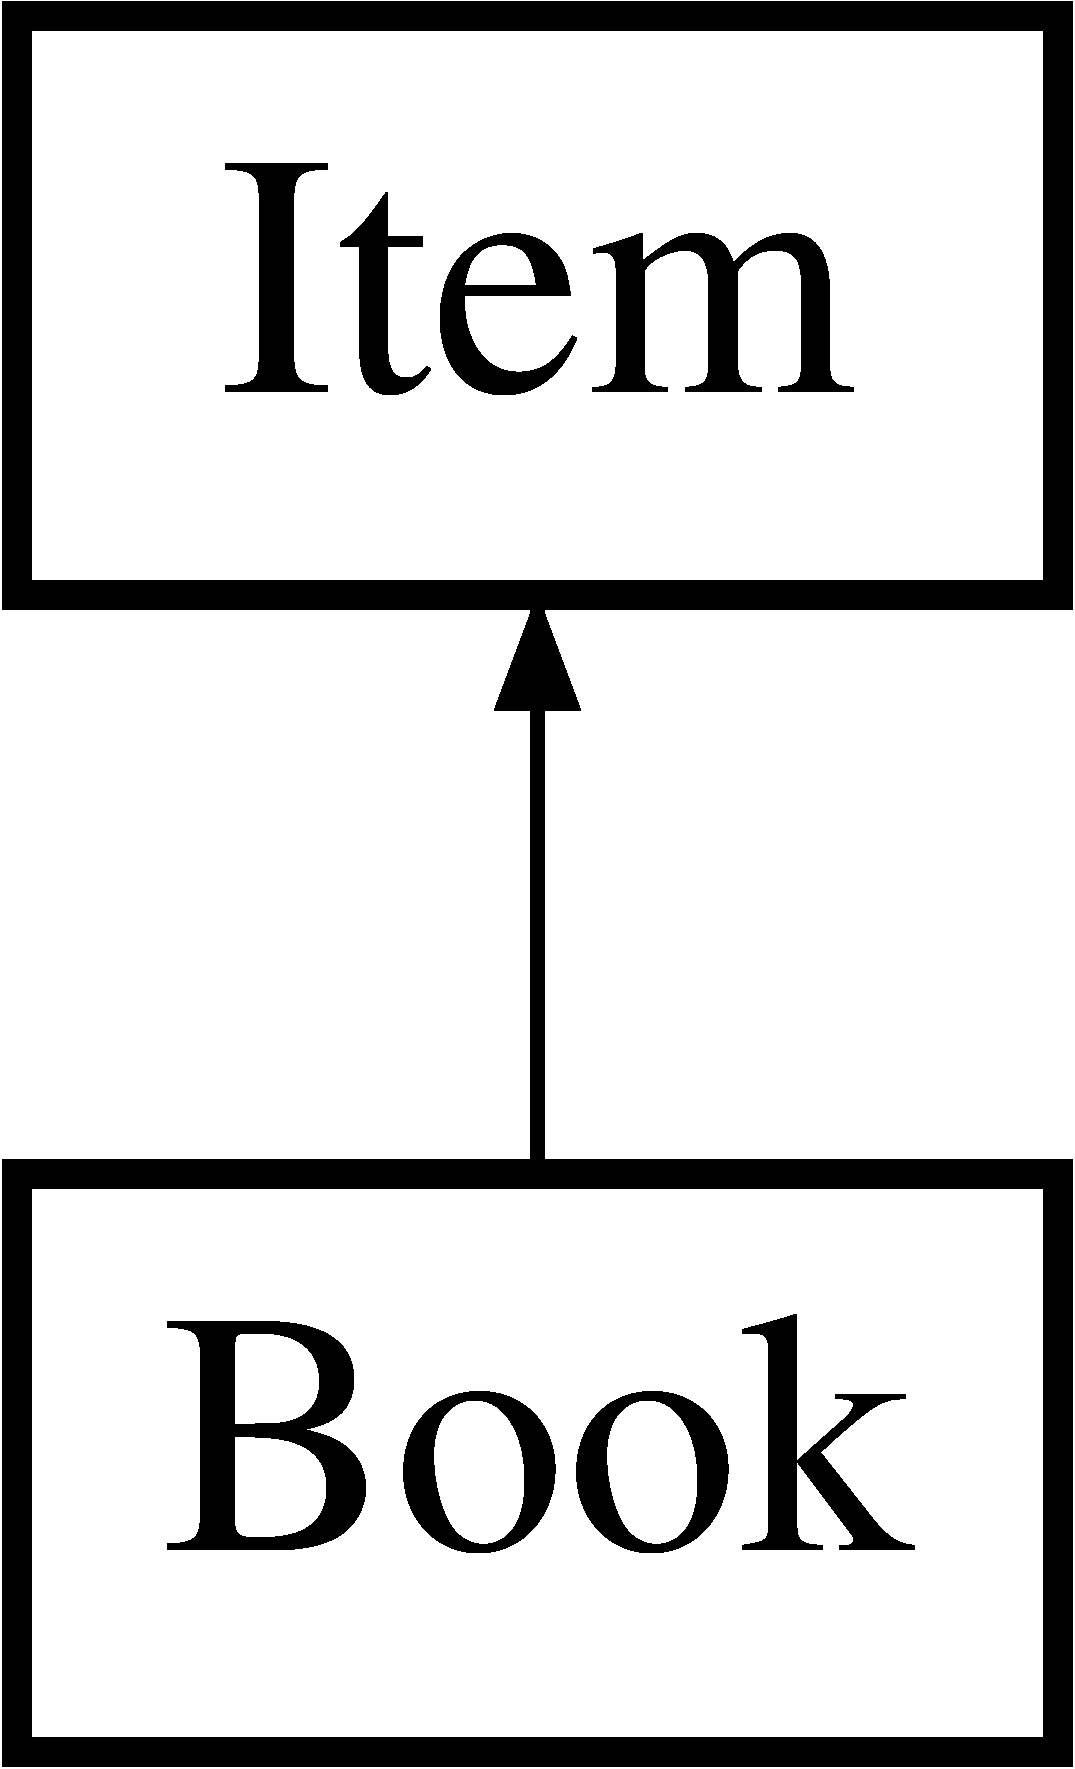
\includegraphics[height=2.000000cm]{class_book}
\end{center}
\end{figure}
\subsection*{Public Member Functions}
\begin{DoxyCompactItemize}
\item 
\hypertarget{class_book_a4aef3c6c555a3c3e4b7c43903add7715}{}{\bfseries Book} (String from\+File)\label{class_book_a4aef3c6c555a3c3e4b7c43903add7715}

\item 
\hypertarget{class_book_a78bd2b22865cf78213049c786aaa32ea}{}String {\bfseries get\+Course} ()\label{class_book_a78bd2b22865cf78213049c786aaa32ea}

\item 
\hypertarget{class_book_a14649f11ec81e6c5b5d59b235160e6a6}{}void {\bfseries print} ()\label{class_book_a14649f11ec81e6c5b5d59b235160e6a6}

\end{DoxyCompactItemize}
\subsection*{Additional Inherited Members}


The documentation for this class was generated from the following file\+:\begin{DoxyCompactItemize}
\item 
Book.\+java\end{DoxyCompactItemize}

\hypertarget{class_course}{}\section{Course Class Reference}
\label{class_course}\index{Course@{Course}}
\subsection*{Public Member Functions}
\begin{DoxyCompactItemize}
\item 
\hypertarget{class_course_abffaf470e0eacdbda2f8e017844f0e36}{}{\bfseries Course} (String from\+File, \hyperlink{class_book}{Book} book)\label{class_course_abffaf470e0eacdbda2f8e017844f0e36}

\item 
\hypertarget{class_course_aa5c333f262e48fd3812814539104ec10}{}void {\bfseries set\+Name} (String name)\label{class_course_aa5c333f262e48fd3812814539104ec10}

\item 
\hypertarget{class_course_aa2c7624b7ad8e9a7005c615dbb43ed9e}{}void {\bfseries set\+Book} (\hyperlink{class_book}{Book} book)\label{class_course_aa2c7624b7ad8e9a7005c615dbb43ed9e}

\item 
\hypertarget{class_course_ae9baad64cf5aec001523fbecb1ee8de7}{}void {\bfseries set\+Hp} (int hp)\label{class_course_ae9baad64cf5aec001523fbecb1ee8de7}

\item 
\hypertarget{class_course_a246738ee9b960276574bca77b96f896c}{}String {\bfseries get\+Name} ()\label{class_course_a246738ee9b960276574bca77b96f896c}

\item 
\hypertarget{class_course_ab769423a99e2e1ebf839837ddf16cb47}{}int {\bfseries get\+Points} ()\label{class_course_ab769423a99e2e1ebf839837ddf16cb47}

\end{DoxyCompactItemize}


The documentation for this class was generated from the following file\+:\begin{DoxyCompactItemize}
\item 
Course.\+java\end{DoxyCompactItemize}

\hypertarget{class_creature}{}\section{Creature Class Reference}
\label{class_creature}\index{Creature@{Creature}}
Inheritance diagram for Creature\+:\begin{figure}[H]
\begin{center}
\leavevmode
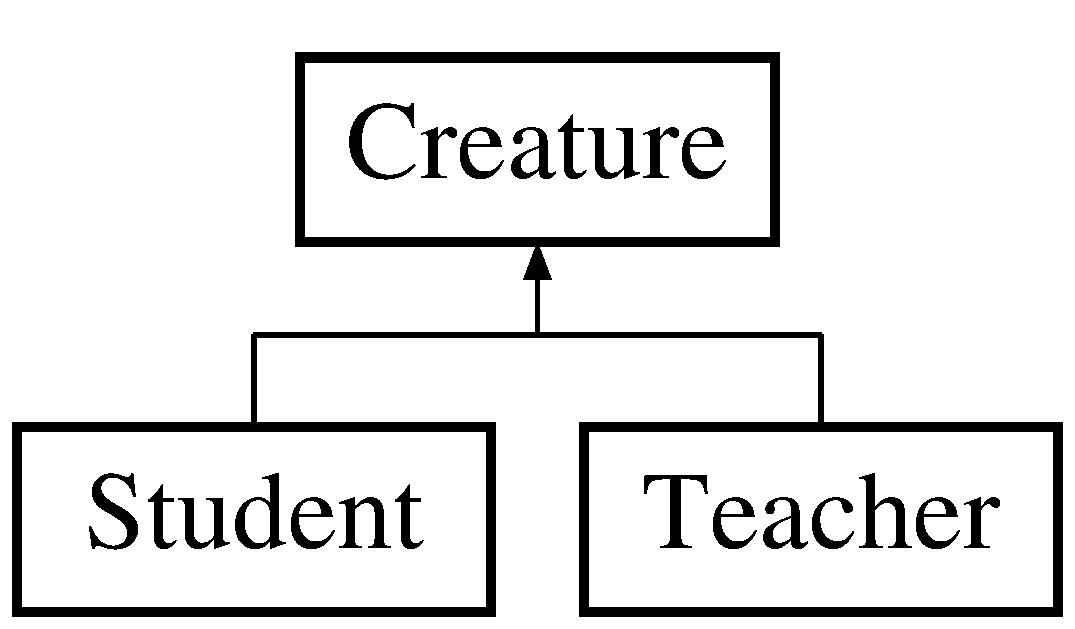
\includegraphics[height=2.000000cm]{class_creature}
\end{center}
\end{figure}
\subsection*{Public Member Functions}
\begin{DoxyCompactItemize}
\item 
\hypertarget{class_creature_a2b52aa516ccf6e45b40d4647330c4741}{}{\bfseries Creature} (String name)\label{class_creature_a2b52aa516ccf6e45b40d4647330c4741}

\item 
\hypertarget{class_creature_ac71e803e8c5f1fe9e88d1b04e96ffa3b}{}String {\bfseries get\+Name} ()\label{class_creature_ac71e803e8c5f1fe9e88d1b04e96ffa3b}

\end{DoxyCompactItemize}
\subsection*{Protected Attributes}
\begin{DoxyCompactItemize}
\item 
\hypertarget{class_creature_a747f9d05acc75973336ea6e9ca126523}{}String {\bfseries name}\label{class_creature_a747f9d05acc75973336ea6e9ca126523}

\end{DoxyCompactItemize}


The documentation for this class was generated from the following file\+:\begin{DoxyCompactItemize}
\item 
Creature.\+java\end{DoxyCompactItemize}

\hypertarget{class_creature_test}{}\section{Creature\+Test Class Reference}
\label{class_creature_test}\index{Creature\+Test@{Creature\+Test}}
\subsection*{Static Public Member Functions}
\begin{DoxyCompactItemize}
\item 
\hypertarget{class_creature_test_a668cae78bfb33180f3401e98d727365b}{}static void {\bfseries main} (String args\mbox{[}$\,$\mbox{]})\label{class_creature_test_a668cae78bfb33180f3401e98d727365b}

\end{DoxyCompactItemize}


The documentation for this class was generated from the following file\+:\begin{DoxyCompactItemize}
\item 
Creature\+Test.\+java\end{DoxyCompactItemize}

\hypertarget{class_gameplay}{}\section{Gameplay Class Reference}
\label{class_gameplay}\index{Gameplay@{Gameplay}}
\subsection*{Static Public Member Functions}
\begin{DoxyCompactItemize}
\item 
\hypertarget{class_gameplay_ab6378a6e29dfbc0f2a977edaa9e05664}{}static void {\bfseries main} (String args\mbox{[}$\,$\mbox{]})\label{class_gameplay_ab6378a6e29dfbc0f2a977edaa9e05664}

\end{DoxyCompactItemize}


The documentation for this class was generated from the following file\+:\begin{DoxyCompactItemize}
\item 
Gameplay.\+java\end{DoxyCompactItemize}

\hypertarget{class_item}{}\section{Item Class Reference}
\label{class_item}\index{Item@{Item}}
Inheritance diagram for Item\+:\begin{figure}[H]
\begin{center}
\leavevmode
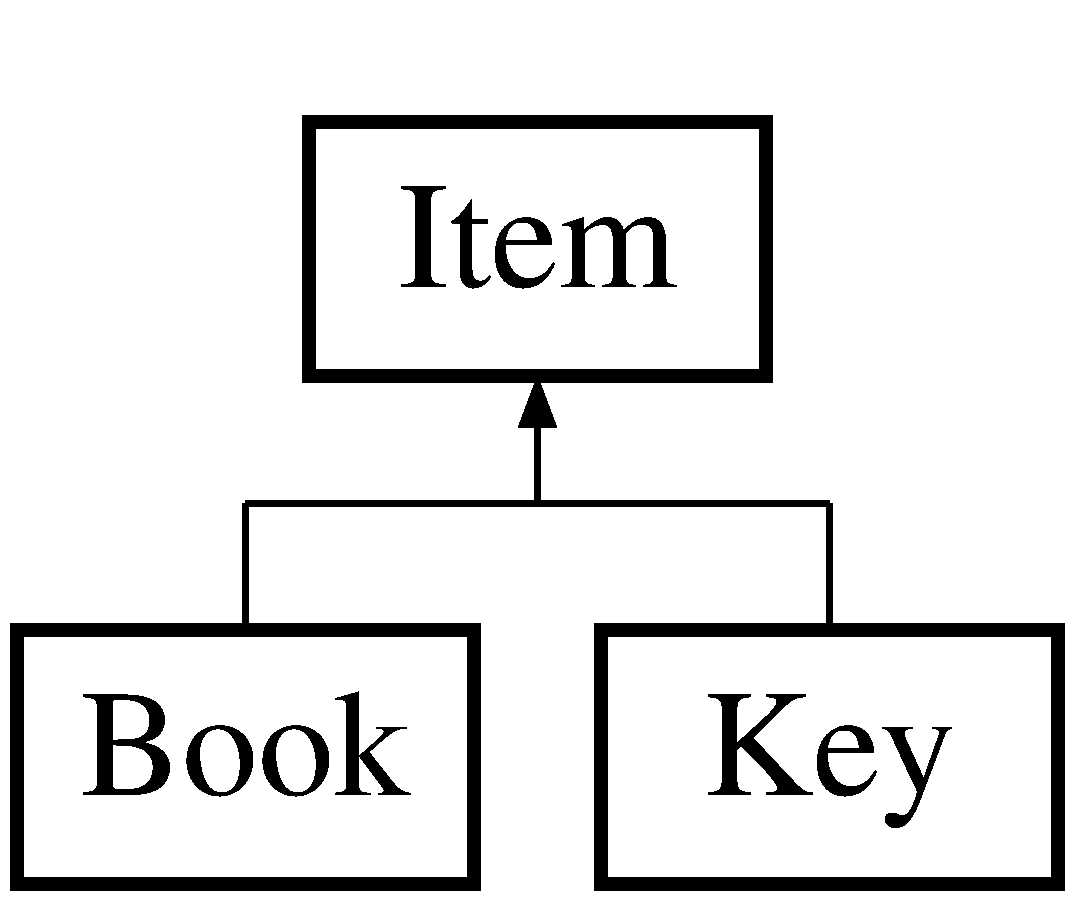
\includegraphics[height=2.000000cm]{class_item}
\end{center}
\end{figure}
\subsection*{Public Member Functions}
\begin{DoxyCompactItemize}
\item 
\hypertarget{class_item_a78dd5a8370c5267c3f1f992167ab84ac}{}String {\bfseries get\+Name} ()\label{class_item_a78dd5a8370c5267c3f1f992167ab84ac}

\item 
\hypertarget{class_item_a639ccc11f3e820d7e39d11d27a00848c}{}int {\bfseries get\+Size} ()\label{class_item_a639ccc11f3e820d7e39d11d27a00848c}

\item 
\hypertarget{class_item_ae3bfa18643ec750ff3d3623b3c120c36}{}void {\bfseries print} ()\label{class_item_ae3bfa18643ec750ff3d3623b3c120c36}

\end{DoxyCompactItemize}
\subsection*{Protected Attributes}
\begin{DoxyCompactItemize}
\item 
\hypertarget{class_item_a42fd6d4796fcf652806278f65ce93a3b}{}String {\bfseries name}\label{class_item_a42fd6d4796fcf652806278f65ce93a3b}

\item 
\hypertarget{class_item_a8629eea6d98387a8c6d4647050feaa84}{}int {\bfseries size}\label{class_item_a8629eea6d98387a8c6d4647050feaa84}

\end{DoxyCompactItemize}


The documentation for this class was generated from the following file\+:\begin{DoxyCompactItemize}
\item 
Item.\+java\end{DoxyCompactItemize}

\hypertarget{class_key}{}\section{Key Class Reference}
\label{class_key}\index{Key@{Key}}
Inheritance diagram for Key\+:\begin{figure}[H]
\begin{center}
\leavevmode
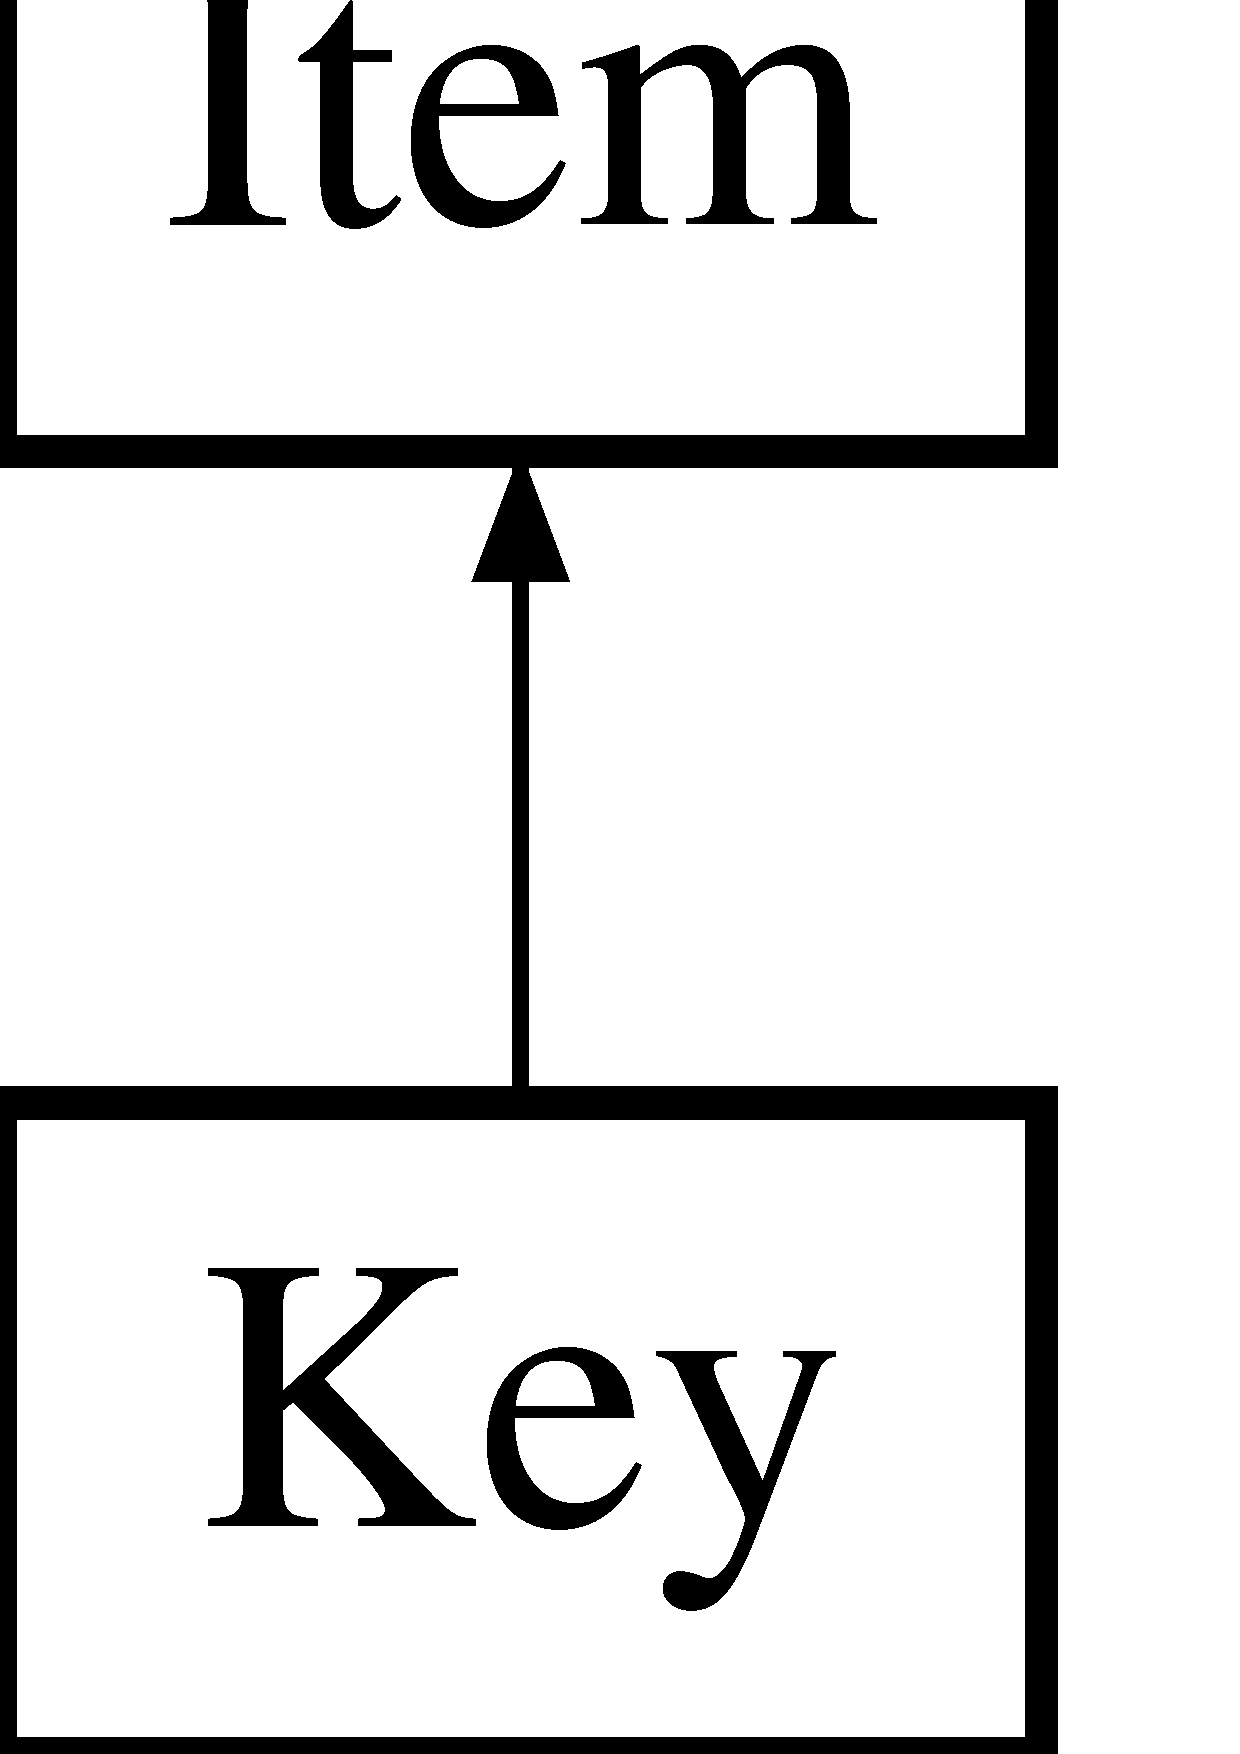
\includegraphics[height=2.000000cm]{class_key}
\end{center}
\end{figure}
\subsection*{Public Member Functions}
\begin{DoxyCompactItemize}
\item 
\hypertarget{class_key_a27c1696c1be29a28f1e75ed7a0dfc2c8}{}{\bfseries Key} (String name)\label{class_key_a27c1696c1be29a28f1e75ed7a0dfc2c8}

\item 
\hypertarget{class_key_aa0d0ff3ecfb5ba587199644fbaeb5bb6}{}boolean {\bfseries use\+Key} ()\label{class_key_aa0d0ff3ecfb5ba587199644fbaeb5bb6}

\item 
\hypertarget{class_key_a467d8f295f185fa716da3db2f9ca8d55}{}void {\bfseries print} ()\label{class_key_a467d8f295f185fa716da3db2f9ca8d55}

\end{DoxyCompactItemize}
\subsection*{Additional Inherited Members}


The documentation for this class was generated from the following file\+:\begin{DoxyCompactItemize}
\item 
Key.\+java\end{DoxyCompactItemize}

\hypertarget{class_room}{}\section{Room Class Reference}
\label{class_room}\index{Room@{Room}}
\subsection*{Public Member Functions}
\begin{DoxyCompactItemize}
\item 
\hypertarget{class_room_a719615305775cef142343f33b59635a7}{}{\bfseries Room} (String room\+Info, \hyperlink{class_creature}{Creature}\mbox{[}$\,$\mbox{]} creature\+List, \hyperlink{class_item}{Item}\mbox{[}$\,$\mbox{]} item\+List)\label{class_room_a719615305775cef142343f33b59635a7}

\item 
\hypertarget{class_room_a9a37ffe731cc4a674b678187c2fafb80}{}void {\bfseries print\+Room\+Creatures} ()\label{class_room_a9a37ffe731cc4a674b678187c2fafb80}

\item 
\hypertarget{class_room_ab638bfd4155075a97e6d3ec306b467f0}{}String {\bfseries get\+Name} ()\label{class_room_ab638bfd4155075a97e6d3ec306b467f0}

\item 
\hypertarget{class_room_a63878e6e7b9ee40f5f826bf723f42eb7}{}void {\bfseries print\+Room\+Items} ()\label{class_room_a63878e6e7b9ee40f5f826bf723f42eb7}

\end{DoxyCompactItemize}


The documentation for this class was generated from the following file\+:\begin{DoxyCompactItemize}
\item 
Room.\+java\end{DoxyCompactItemize}

\hypertarget{class_room_test}{}\section{Room\+Test Class Reference}
\label{class_room_test}\index{Room\+Test@{Room\+Test}}
\subsection*{Static Public Member Functions}
\begin{DoxyCompactItemize}
\item 
\hypertarget{class_room_test_aaaf731386801063462f02a1d77f132d3}{}static void {\bfseries main} (String args\mbox{[}$\,$\mbox{]})\label{class_room_test_aaaf731386801063462f02a1d77f132d3}

\end{DoxyCompactItemize}


The documentation for this class was generated from the following file\+:\begin{DoxyCompactItemize}
\item 
Room\+Test.\+java\end{DoxyCompactItemize}

\hypertarget{class_sfinxen}{}\section{Sfinxen Class Reference}
\label{class_sfinxen}\index{Sfinxen@{Sfinxen}}
\subsection*{Public Member Functions}
\begin{DoxyCompactItemize}
\item 
\hypertarget{class_sfinxen_a8aca78bdc58a388ee023a2cf1055fab3}{}{\bfseries Sfinxen} (String\mbox{[}$\,$\mbox{]} wisdom\+Words, int points\+To\+Graduate)\label{class_sfinxen_a8aca78bdc58a388ee023a2cf1055fab3}

\item 
\hypertarget{class_sfinxen_a873e3e3f24ca14bbfe32b5a3abd3f128}{}void {\bfseries talk} ()\label{class_sfinxen_a873e3e3f24ca14bbfe32b5a3abd3f128}

\item 
\hypertarget{class_sfinxen_a9c3a358e593e12655bc2ef1e44ba984e}{}boolean {\bfseries graduate} (\hyperlink{class_avatar}{Avatar} avatar)\label{class_sfinxen_a9c3a358e593e12655bc2ef1e44ba984e}

\end{DoxyCompactItemize}


The documentation for this class was generated from the following file\+:\begin{DoxyCompactItemize}
\item 
Sfinxen.\+java\end{DoxyCompactItemize}

\hypertarget{class_sfinxen_test}{}\section{Sfinxen\+Test Class Reference}
\label{class_sfinxen_test}\index{Sfinxen\+Test@{Sfinxen\+Test}}
\subsection*{Static Public Member Functions}
\begin{DoxyCompactItemize}
\item 
\hypertarget{class_sfinxen_test_a3a65eaddc58d31428337f4fabd0125a2}{}static void {\bfseries main} (String args\mbox{[}$\,$\mbox{]})\label{class_sfinxen_test_a3a65eaddc58d31428337f4fabd0125a2}

\end{DoxyCompactItemize}


The documentation for this class was generated from the following file\+:\begin{DoxyCompactItemize}
\item 
Sfinxen\+Test.\+java\end{DoxyCompactItemize}

\hypertarget{class_student}{}\section{Student Class Reference}
\label{class_student}\index{Student@{Student}}
Inheritance diagram for Student\+:\begin{figure}[H]
\begin{center}
\leavevmode
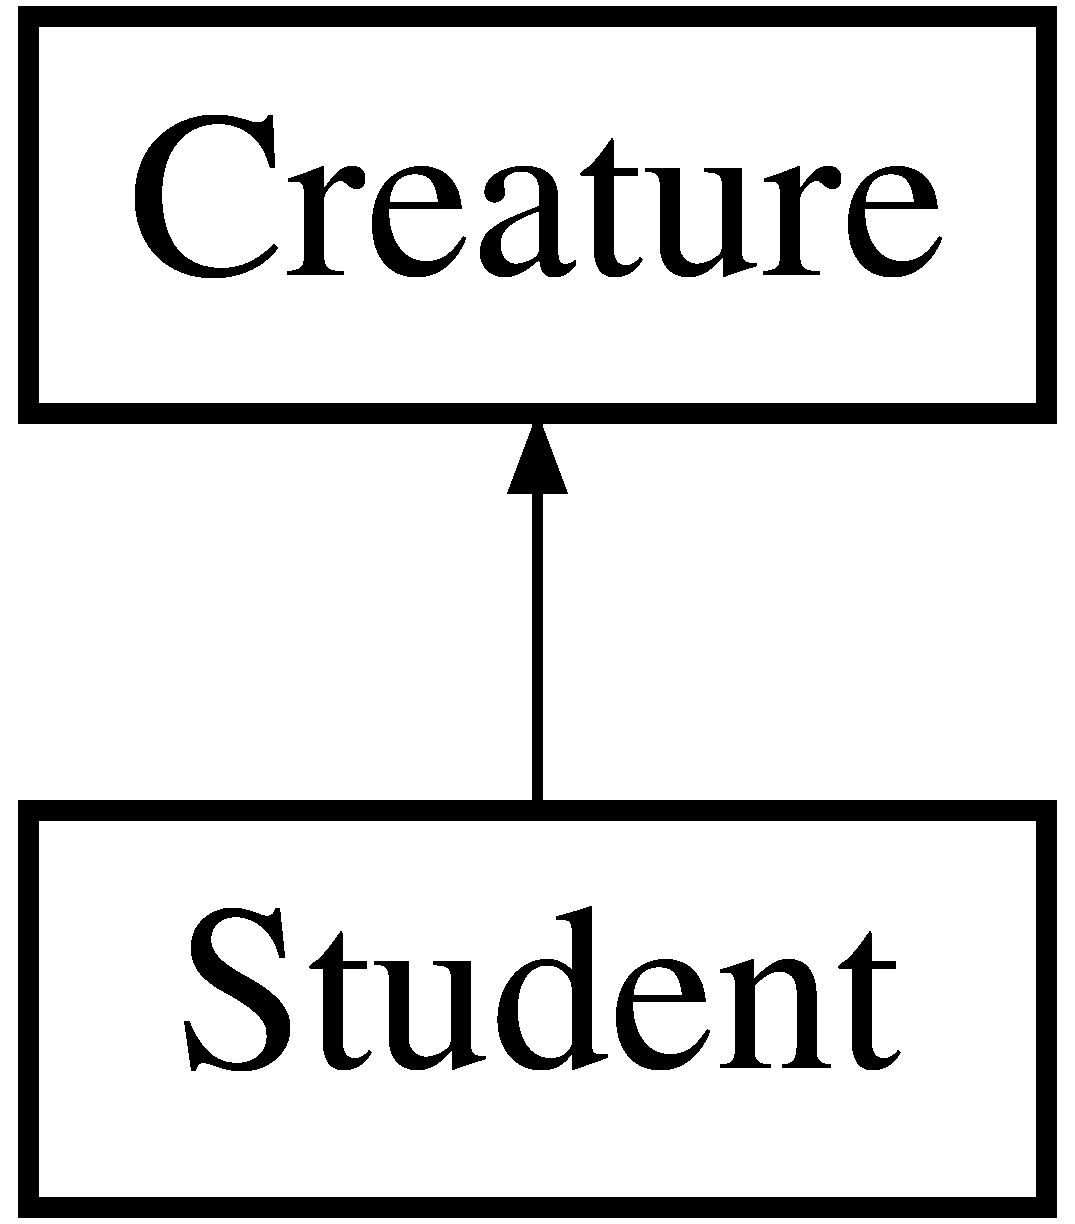
\includegraphics[height=2.000000cm]{class_student}
\end{center}
\end{figure}
\subsection*{Public Member Functions}
\begin{DoxyCompactItemize}
\item 
\hypertarget{class_student_af836d4d8e20f567a6837a1fe16e79ac7}{}{\bfseries Student} (String name, String active\+Course, \hyperlink{class_book}{Book} old\+Book)\label{class_student_af836d4d8e20f567a6837a1fe16e79ac7}

\item 
\hypertarget{class_student_a9b84dc1d537780b4d225dc0318adc75d}{}\hyperlink{class_book}{Book} {\bfseries trade\+Book} (\hyperlink{class_book}{Book} offered\+Book)\label{class_student_a9b84dc1d537780b4d225dc0318adc75d}

\item 
\hypertarget{class_student_a1417ab7f2dd79ed1608833f80a5e5bfa}{}\hyperlink{class_book}{Book} {\bfseries question\+Book} ()\label{class_student_a1417ab7f2dd79ed1608833f80a5e5bfa}

\item 
\hypertarget{class_student_a37a0ad9f33a5b49247eb8d3301887b73}{}String {\bfseries question\+Course} ()\label{class_student_a37a0ad9f33a5b49247eb8d3301887b73}

\end{DoxyCompactItemize}
\subsection*{Additional Inherited Members}


The documentation for this class was generated from the following file\+:\begin{DoxyCompactItemize}
\item 
Student.\+java\end{DoxyCompactItemize}

\hypertarget{class_teacher}{}\section{Teacher Class Reference}
\label{class_teacher}\index{Teacher@{Teacher}}
Inheritance diagram for Teacher\+:\begin{figure}[H]
\begin{center}
\leavevmode
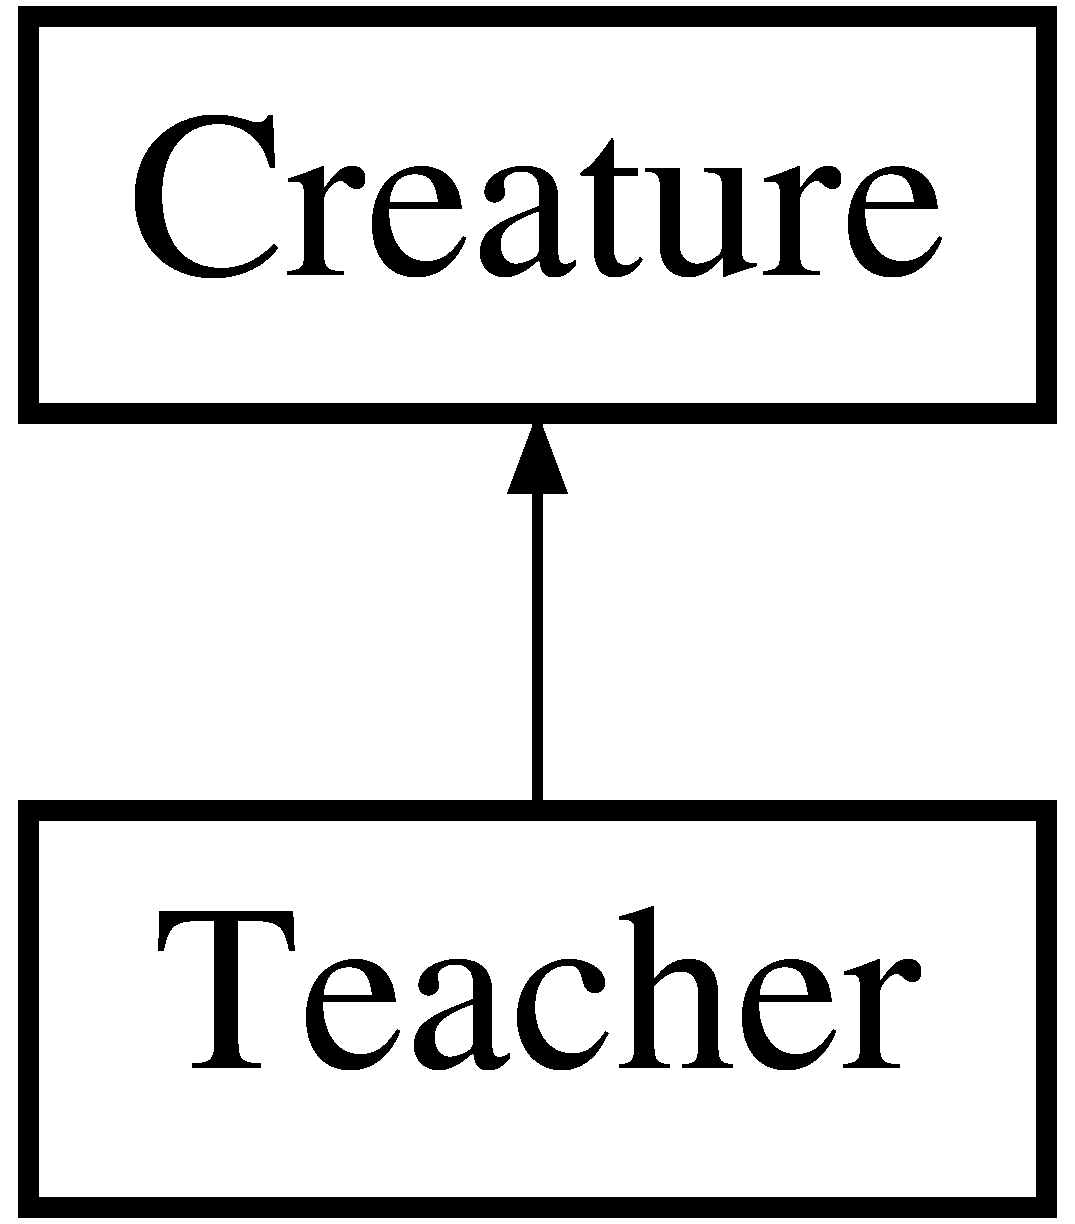
\includegraphics[height=2.000000cm]{class_teacher}
\end{center}
\end{figure}
\subsection*{Public Member Functions}
\begin{DoxyCompactItemize}
\item 
\hypertarget{class_teacher_afe19b71773265eb94a4affa2540b4c6e}{}{\bfseries Teacher} (String name, \hyperlink{class_course}{Course} course, String answers\mbox{[}$\,$\mbox{]}, String question, int right\+Answer)\label{class_teacher_afe19b71773265eb94a4affa2540b4c6e}

\item 
\hypertarget{class_teacher_a009cd73ce30da1e37ce73fcf809b667a}{}\hyperlink{class_course}{Course} {\bfseries get\+Course} ()\label{class_teacher_a009cd73ce30da1e37ce73fcf809b667a}

\item 
\hypertarget{class_teacher_a5de26864d6efad58855d6b387cbcb3d7}{}boolean {\bfseries ask\+Question} (boolean has\+Book)\label{class_teacher_a5de26864d6efad58855d6b387cbcb3d7}

\end{DoxyCompactItemize}
\subsection*{Additional Inherited Members}


The documentation for this class was generated from the following file\+:\begin{DoxyCompactItemize}
\item 
Teacher.\+java\end{DoxyCompactItemize}

\hypertarget{class_world}{}\section{World Class Reference}
\label{class_world}\index{World@{World}}
\subsection*{Public Member Functions}
\begin{DoxyCompactItemize}
\item 
\hypertarget{class_world_a3d74182a02c917b50af9bda00e89fc3c}{}Array\+List$<$ String $>$ {\bfseries load\+File} (String file\+Name)\label{class_world_a3d74182a02c917b50af9bda00e89fc3c}

\item 
\hypertarget{class_world_ae0e0dbf23aa39e948dc4dd9789615c9c}{}\hyperlink{class_course}{Course}\mbox{[}$\,$\mbox{]} {\bfseries return\+First80} ()\label{class_world_ae0e0dbf23aa39e948dc4dd9789615c9c}

\end{DoxyCompactItemize}


The documentation for this class was generated from the following file\+:\begin{DoxyCompactItemize}
\item 
World.\+java\end{DoxyCompactItemize}

\hypertarget{class_world_test}{}\section{World\+Test Class Reference}
\label{class_world_test}\index{World\+Test@{World\+Test}}
\subsection*{Public Member Functions}
\begin{DoxyCompactItemize}
\item 
\hypertarget{class_world_test_a51f1814bf8bfec8588f5fe6c2a269679}{}void {\bfseries test\+Load\+File} ()\label{class_world_test_a51f1814bf8bfec8588f5fe6c2a269679}

\end{DoxyCompactItemize}


The documentation for this class was generated from the following file\+:\begin{DoxyCompactItemize}
\item 
World\+Test.\+java\end{DoxyCompactItemize}

%--- End generated contents ---

% Index
\backmatter
\newpage
\phantomsection
\clearemptydoublepage
\addcontentsline{toc}{chapter}{Index}
\printindex

\end{document}
